\documentclass[12pt, letterpaper]{article}
\usepackage[utf8]{inputenc}
\usepackage{apacite}
\usepackage{fullpage}
\usepackage{indentfirst}
\usepackage{enumerate}
\usepackage{amsmath}
\usepackage{graphicx}
\graphicspath{ {./images/} }
\usepackage{wrapfig}
\usepackage[table]{xcolor}
\usepackage{float}
\restylefloat{table}

\title{
    Acea Smart Water Analytics \\
    \large MATH 189 Group 2 Final Project}
\author{
    Kasen Teoh, 
    Chung En Pan, 
    Nathan Fallahi, \\
    Parsa Ganjooi, 
    and Eamon Jarrett-Mann
}
\date{Winter 2021}

\begin{document}
\maketitle

\section{Introduction}
Every day the number of humans on the planet continues to rise and with it, the consumption of natural resources, such as water. As humans, we use tens, if not hundreds, of gallons of water a day, in the restroom, kitchen, garden, and simply drinking. While it may seem like there is an abundance of water, mainly the oceans, we require fresh water, water from aquifers, springs, lakes, and rivers to sustain our lives. With the increasing amount of life on the planet, we need to make strategic decisions regarding where water should be extracted from and how to ration water portions to allow the water source to last. For instance, if a particular waterbody was close to being drained and we knew it would not quickly replenish naturally, we could avoid using the last of the water. Additionally, in different seasons, such as spring and summer, where rainfall might be scarce, conservation of water is critical. In this project, we aim to analyze water availability in four different types of water bodies, aquifers, springs, rivers, and lakes, and attempt to predict the availability on a daily basis. To achieve this analysis, we break our goal into several parts:
\begin{enumerate}
    \item Analyze the seasonal rainfall throughout the entirety of the study by using both graphical visualizations and interval estimates of seasonal rainfall 
    \item Analyze the connections between the variables in the dataset and the variables to predict (Depth to groundwater for aquifers, flow rate for springs, lake level and flow rate for lakes, and hydrometry for rivers). Here, we can also identify which variables affect the outcome variables significantly
    \item Determine whether a linear regression model is suitable for the datasets in question
\end{enumerate}

\section{Data}
Our data was sourced from a Kaggle Analytics Competition \cite{acea2020}. There are a total of nine datasets consisting of four aquifers, three springs, one lake, and one river which each contain various features. Not all days have the same measurements as some features were only recorded for certain dates. All datasets have measurements from a specific date until June 6, 2020. Each measurement includes the date it was measured on as a variable. For all the datasets, rainfall is measured in millimeters, depth to groundwater in meters,  temperature in degrees Celsius, volume in cubic meters, hydrometry (groundwater level) in meters, flow rate in cubic meters per second, and lake level (river water level) in meters. All measurements/features are continuous numerical variables, except for the date which is discrete and numerical.

The Auser aquifer dataset has measurements for 8,154 days since 1998. There are measurements of rainfall at 10 locations, depth to rainfall at 5 locations, temperature at 4 locations, volume at 5 locations, and hydrometry at 2 locations. The Doganella aquifer dataset has measurements for 6,026 days since 2004. There are 2 rainfall, 9 depth to groundwater, 9 volume, and 2 temperature measurements. The Luco aquifer dataset has measurements for 7,487 days since 2000. There are 10 rainfall, 4 depth to groundwater, 4 temperature, and 4 volume measurements. The Petrignano aquifer dataset has measurements for 5,223 days since 2006. There are 1 rainfall, 2 depth to groundwater, 2 temperature, 1 volume, and 1 hydrometry measurements. 

The Bilancino lake dataset has measurements for 6,603 days since 2002. There are 5 rainfall, 1 temperature, 1 lake level, and 1 flow rate measurements. 

The Arno river dataset has measurements for 8,217 days since 1998. There are 14 rainfall, 1 temperature, and 1 hydrometry measurements.

The Amiata water spring dataset has measurements for 7,487 days since 2000. There are 5 rainfall, 3 depth to groundwater, 3 temperature, and 4 flow rate measurements. The Lupa water spring dataset has measurements for 4,199 days since 2009. There is 1 rainfall and 1 flow rate measurement. The Madonna di Canneto water spring dataset has measurements for 3,113 days since 2012. There is 1 rainfall, 1 temperature, and 1 flow rate measurement.

\section{Background}
Water availability is defined as the amount of water that humans can extract without harmful repercussions to the ecosystem and other organisms. This is basically saying how much water can we use without harming the environment or organisms that live in the environment.

An aquifer is a body of rock or sediment that holds groundwater. Groundwater is the precipitation that has combined with the soil below the surface and collected in empty spaces underground. Most groundwater, including a significant amount of our drinking water, comes from aquifers. In order to access the groundwater, a well must be created by drilling a hole that reaches the aquifer. While wells extract water from aquifers, aquifers also flow to other springs. If groundwater abstraction exceeds groundwater recharge for extensive areas and long time, overexploitation or persistent groundwater depletion can occur \cite{gleeson2010commentary}. Since the 1960s groundwater abstraction has more than doubled, resulting in an increase in groundwater depletion. \cite{wada2010global}. From the 1960’s to 2010, the demand for groundwater had doubled, consequently the abstraction of groundwater doubled, leading to a depletion of groundwater. If this rate continues, we will have depleted our groundwater resources in the near future. 

According to the US Geology Survey, a spring is a water resource formed from an aquifer being filled to the point that the water overflows onto the land surface. Because springs are derived from when aquifers’ groundwater reaches the surface, the depletion of groundwater directly impacts springs. With the disappearance of aquifers and groundwater, there is no more water underground to flow to springs, and hence, the disappearance of springs follows. For instance, in the Nubian Aquifer system about 25\% of the total withdrawals in 1998 resulted in reductions in natural flow to other water bodies, such as springs and oases \cite{cedare2001}. 

Lakes are bodies of water that are surrounded by land. If a lake flows into a river or ocean, it is considered an opened lake while if it does not flow into another water body, it is considered closed. Lakes’ water supplies are replenished through groundwater seepage and/or natural means, i.e rain, snow, etc. Many organisms, not limited to just humans, depend on lakes as a cornerstone of life: fish, plants, birds, and etc.  According to Inland water loss in the Aral Sea, Lake Urmia, the Great Salt Lake, Lake Abert, and Lake Poopo accounts for more than half of total inland water loss in terminal lakes on several of Earth's continents \cite{wine2020water}.

A river is a natural flowing body of water that flows towards oceans, lakes, or other rivers. Every drop of water in rivers flowing across the land once fell to Earth from the atmosphere and given enough time, every drop will return to the atmosphere as water vapor \cite{karr1998restoring}. However, if humans continue down the current path and are not wise about the extraction of water, rivers could dry up permanently, further depleting the resource. Retaining the biological parts of riverine ecosystems, as well as the processes that nourish them is crucial to retaining water supplies and all the goods and services associated with water \cite{karr1998restoring}. 

These four water bodies are essential to human life. While there are many more water bodies, such as oceans, we aim to highlight which season would be the smartest time to extract water from each of these four water bodies, allowing for the continuation for human growth, while also maintaining a hospitable ecosystem for other life and organisms as well. 

\section{Analysis}
\subsection{Aquifers}
For Aquifers we have a total of four datasets: Auser, Petrigano, Doganella, and Luco.
\subsubsection{Auser}
The Auser aquifer consists of two subsystems, north and south. The north subsystem is a water table (or unconfined) aquifer while the south subsystem is an artesian (or confined) groundwater. The north subsystem partly influences the behavior of the south subsystem.

\begin{figure}[H]
    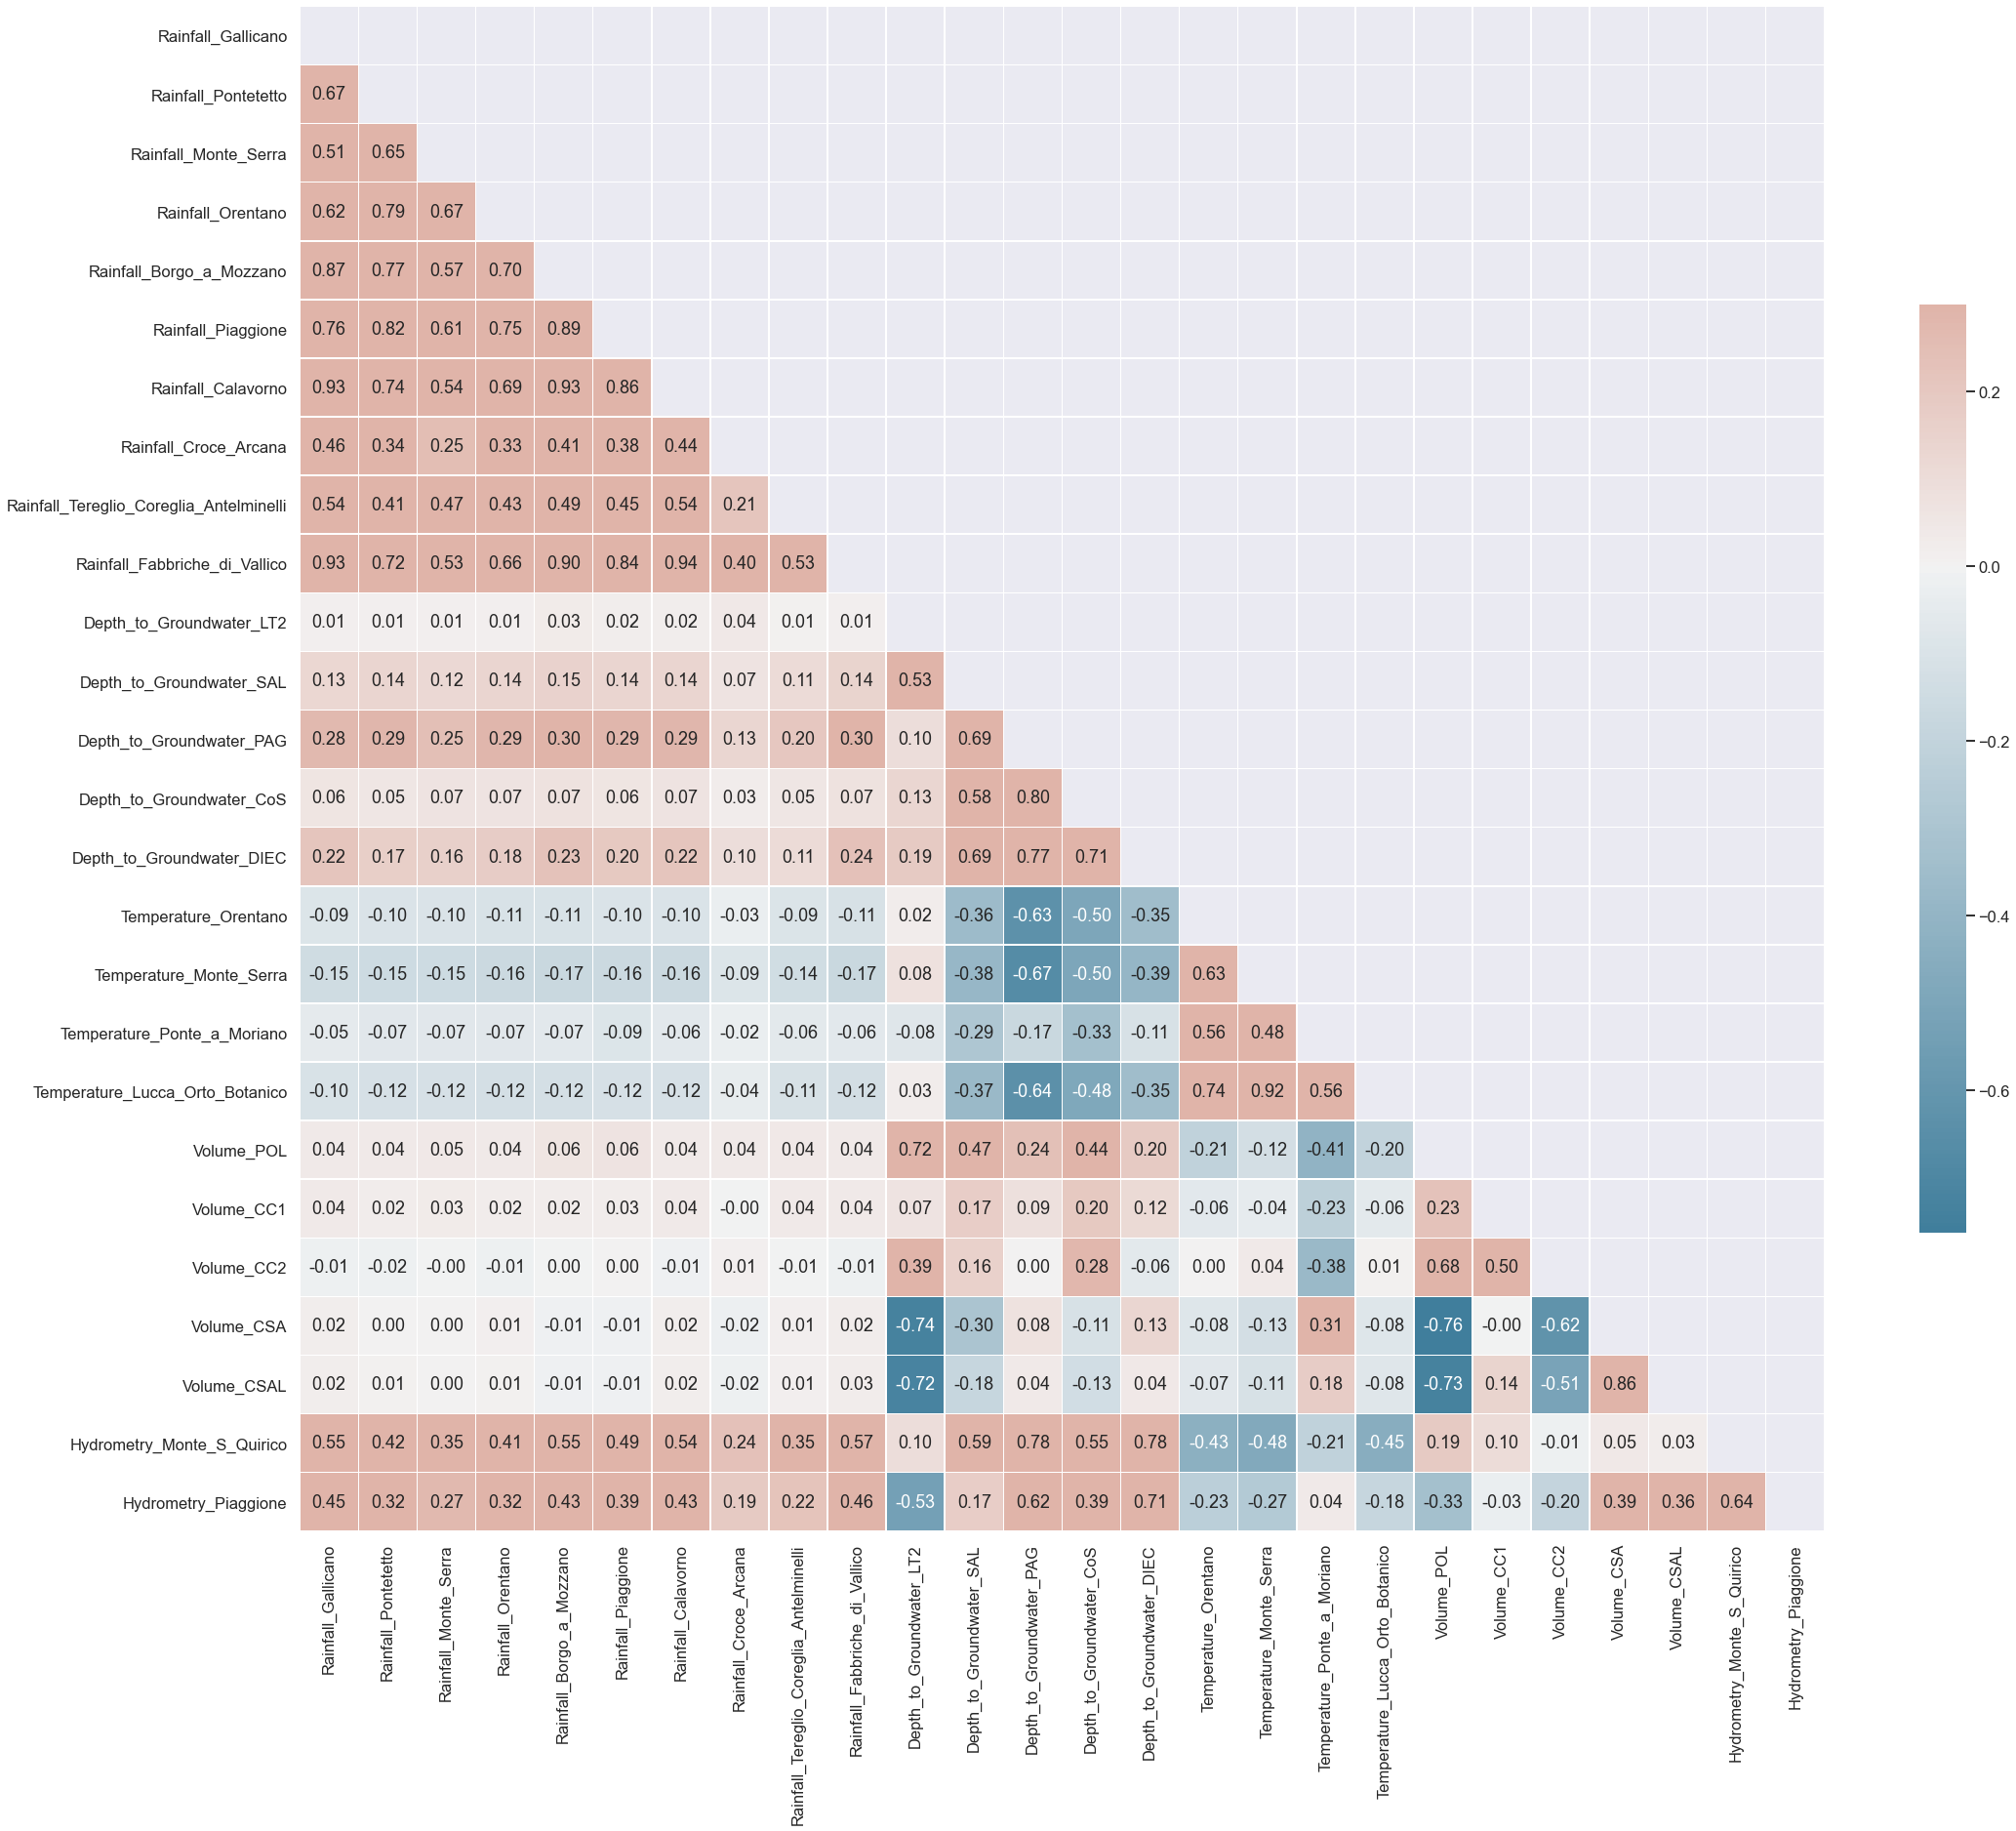
\includegraphics[width=1\textwidth]{aq_auser_heatmap.png}
    \centering
\end{figure}

This heatmap shows a correlation matrix for all the variables in the Auser aquifer dataset. As you can see, many of the rainfalls are correlated across regions, which makes sense as they are likely close to each other. Additionally, it seems like the depth to groundwater (outcome) measures are not well correlated with other features other than the other depths to groundwater.

\begin{figure}[H]
    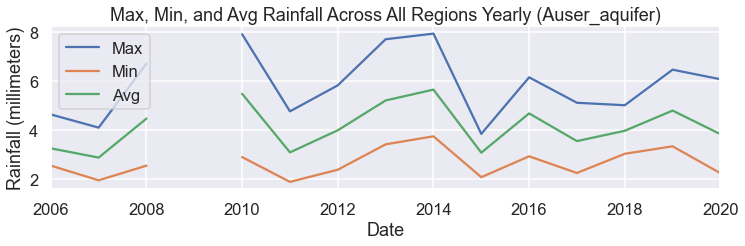
\includegraphics[width=1\textwidth]{aq_auser_maxminavg.png}
    \centering
\end{figure}

As you can see above, the Auser aquifer has a wide variety of rainfall meaures, with some years receiving as much as 5 mm on average and other years staying much drier with half the volume of rainfall. This graph gives a good idea of how the rainfall changes from year to year. Additionally, we see that there was no data collected in the year 2009. 

\begin{verbatim}
TODO: add rest of table
\end{verbatim}

\begin{table}[H]
    \rowcolors{2}{gray!20}{white}
    \begin{tabular}{r|cccc}
    \textbf{Region}                 & \textbf{Winter}    & \textbf{Spring}    & \textbf{Summer}    & \textbf{Autumn}    \\ \hline
    \textbf{Rainfall\_Gallicano}    & {[}6.003, 7.76{]}  & {[}1.501, 1.94{]}  & {[}3.002, 3.88{]}  & {[}4.502, 5.82{]}  \\
    \textbf{Rainfall\_Pontetto}     & {[}4.248, 5.505{]} & {[}1.062, 1.376{]} & {[}2.124, 2.753{]} & {[}3.186, 4.129{]} \\
    \textbf{Rainfall\_Monte\_Serra} & {[}4.797, 6.269{]} & {[}1.199, 1.567{]} & {[}2.399, 3.134{]} & {[}3.598, 4.702{]}
    \end{tabular}
    \centering
\end{table}

Above, we see the generated prediction intervals of the estimated seasonal rainfall, temperature, volume, and hydrometry. Using these prediction intervals along with the correlations and regression coefficients will allow us to determine what affects the depth to groundwater the most and what season will be optimal for water extraction.
        
\begin{verbatim}
Linear regression PCA models for Auser_aquifer
    RMSE when predicting the Depth_to_Groundwater_LT2 1.144
    RMSE when predicting the Depth_to_Groundwater_SAL 1.131
    RMSE when predicting the Depth_to_Groundwater_PAG 0.805
    RMSE when predicting the Depth_to_Groundwater_CoS 2.074
    RMSE when predicting the Depth_to_Groundwater_DIEC 0.777
\end{verbatim}

When predicting depth to ground water using linear regression models, there is a bit of error for all depths, but CoS is significantly worse (about 2x as much error) than any of the other presented linear regression models.

\begin{figure}[H]
    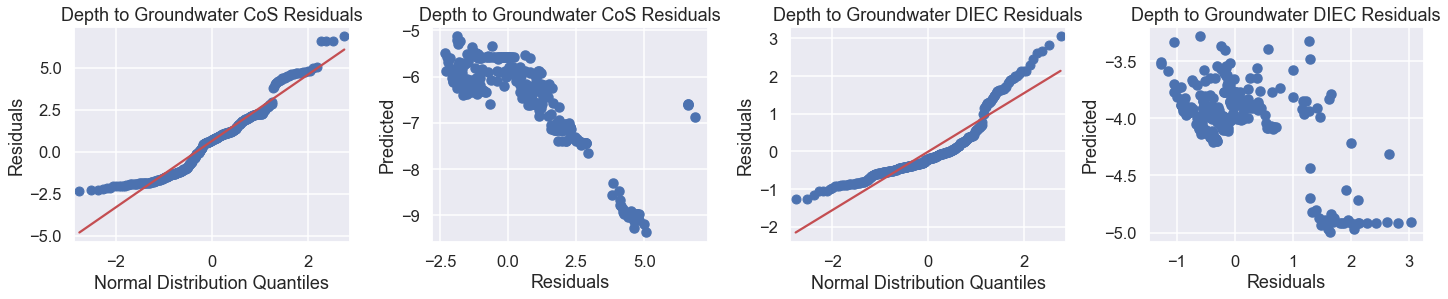
\includegraphics[width=1\textwidth]{aq_auser_residuals.png}
    \centering
\end{figure}

Above, we see two of the five residual plots. In both cases, we see that the distribution of the residuals does not follow a normal distribution. The Cos residuals scatter plots shows a negative sloped scatter plot while the DIEC residuals scatter plots dot not should much of an obvious patter and is somewhat centered around 0.

\begin{verbatim}
TODO: Predicting Depth to Groundwater table goes here.
\end{verbatim}

As you can see from the tables above, most of the features in the dataset are not strongly correlated with the varied depth outcomes. Above, we displayed two out of the five coefficients as they were relatively similar. In fact, even the other depths are not strongly correlated with the depth outcomes, and many are not statistically significant. The two constant and strong correlated throughout all five regression models was the rainfall in the regions of Gallicano and Pontetto. This was not too surprising as the these two were constantly held the highest Pearson correlation coefficient with the depth to ground water variables. 

\subsubsection{Petrigano}
The Petrigano aquifer is water table groundwater and is also fed by the Chiascio river. The grounderwater levels are influences by rainfall, depth to groundwater, temperatures, drainage volumes, and level of the Chiascio river.

\begin{table}[H]
    \rowcolors{2}{gray!20}{white}
    \begin{tabular}{ll}
    \textbf{Variable}                       & \textbf{Non-Null Count} \\ \hline
    Rainfall\_Bastia\_Umbra                 & 4199                    \\
    Depth\_to\_Groundwater\_P24             & 5168                    \\
    Depth\_to\_Groundwater\_P25             & 5184                    \\
    Temperature\_Bastia\_Umbra              & 4199                    \\
    Temperature\_Petrignano                 & 4199                    \\
    Volume\_C10\_Petrignano                 & 5025                    \\
    Hydrometry\_Fiume\_Chiascio\_Petrignano & 4199                   
    \end{tabular}
    \centering
\end{table}

Above we see that this is one of the few complete datasets that we are given. For the predictor variables we have between 4000-5000 observations and for the outcome variables we have around 5000 observations. Hence, we do not need to drop any big pieces of data.

\begin{figure}[H]
    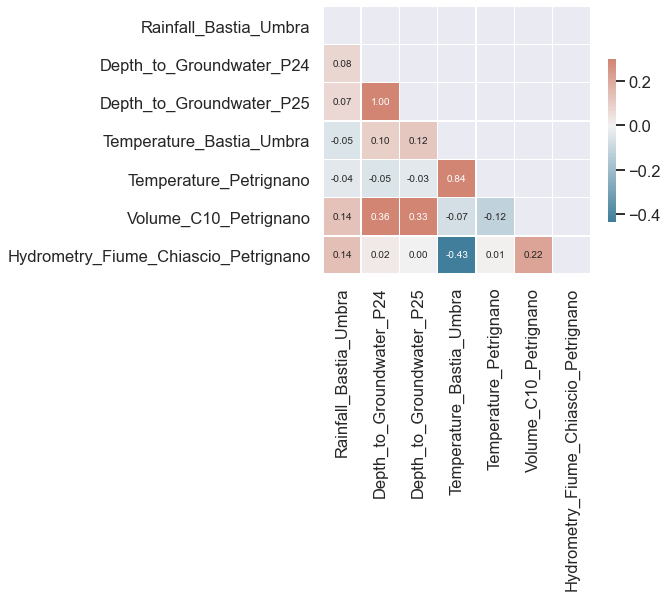
\includegraphics[width=.75\textwidth]{aq_petrigano_heatmap.png}
    \centering
\end{figure}

As you can see from the heatmap above, many of the rainfalls are correlated across regions, which makes sense as they are likely close to each other. Additionally, it seems like the depth to groundwater (outcome) measures are not well correlated with other features other than the other depths to groundwater.

\begin{figure}[H]
    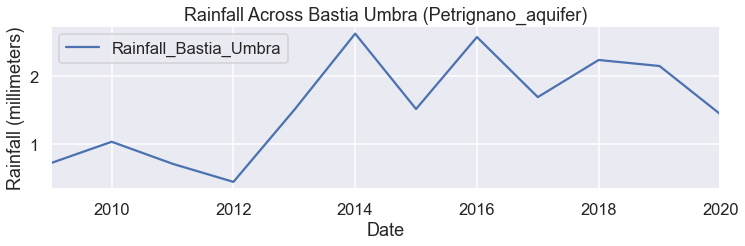
\includegraphics[width=.75\textwidth]{aq_petrigano_rainfall.png}
    \centering
\end{figure}

As you can see above, the petrignano aquifer has a less variety of rainfall meaures than most of the other aquifers, with values between .5mm and 2.5 mm. This graph gives a good idea of how the rainfall changes from year to year, and seems relatively consistent with the Auser number as 2014 is a relatively wet year in these regions as well.

\begin{verbatim}
TODO: prediction interval tables
\end{verbatim}

Above is the prediction intervals for the Petrignano aquifer. We see that in the Summer and Autumn months, the rainfall is fairly constant while in the Winter is could be double.

\begin{verbatim}
Linear regression PCA models for Petrignano_aquifer
    RMSE when predicting the Depth_to_Groundwater_P24 2.339
    RMSE when predicting the Depth_to_Groundwater_P25 2.234
\end{verbatim}

As you can see above, the RMSE for these models is uniformly higher than the presented models for the Auser aquifer.

\begin{figure}[H]
    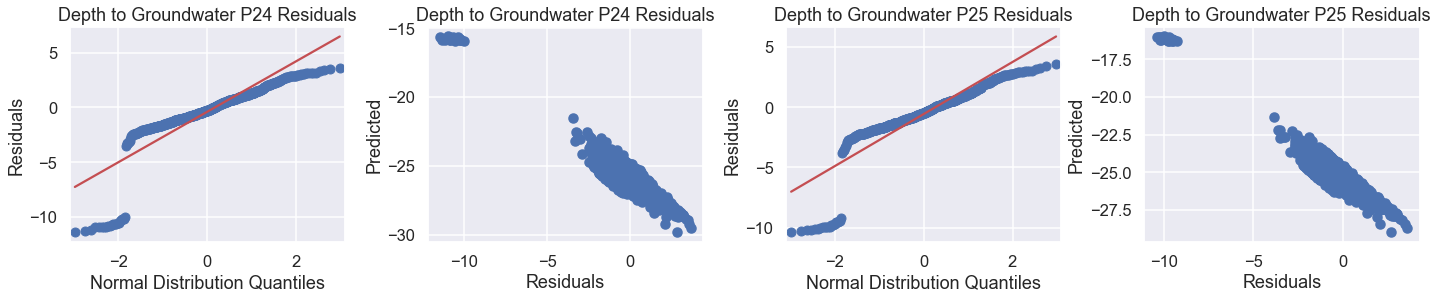
\includegraphics[width=.75\textwidth]{aq_petrigano_residuals.png}
    \centering
\end{figure}

Once again, we see that the residuals are not normally distributed and not randomly scatted. This leads us to believe that a linear model is not suitable for our data.

\begin{verbatim}
TODO: Predicting Depth to Groundwater at P24 tables
\end{verbatim}

The Petrignano aquifer only has 2 depth measures, both of which have strong negative correlation with rainfall in Bastia Umbra and a small amount of negative correlation with the temperature in the Petrignano region. Further, there is a small amount of spositive correlation with the Volume c10 Petrignano. As you can see, there is little correlation with any of the other features present in the dataset.

\subsubsection{Doganella}

\subsubsection{Luco}

\subsection{Water Springs}
\subsubsection{Amiata}

\subsubsection{Lupa and Madonna di Canneto}

\subsection{Lakes}
\subsection{Rivers}

\section{Limitations}
In our analysis, there were some limitations. For all of the datasets, there were at minimum, a few hundred missing observations. In some cases, many variables were missing more than half of the years the study was performed. In these cases, we had decided to drop the variables entirely. When there were just a few missing observations within a variable, we had dropped that observation entirely because we had decided that imputing the missing data may lead to biased results. This would not represent an accurate interpretation of the data set.

Another factor that may have decreased our model’s power is multicollinearity. In many of our datasets, there were multiple variables with strong correlation, and occasionally, perfect correlation among each other. Because multicollinearity affects the way we interpret our model, we had attempted to utilize principal component analysis to reduce the number of components used in our linear regression. In most cases, the particular dataset’s variance was able to be explained in using half the number of the principal components. 

One of the most important limitations in our analysis is the linear regression model. Our dataset is a time-series data, meaning that the observations within the data are not independent. While linear regression is usually not the best choice when predicting time-series data, a linear regression model may be suitable if the residuals of the linear model are normally distributed and do not show a pattern. When we trained and tested our model, a few of our residuals were normally distributed while the others were not and the spread of the residuals were often in groups. Because of this, we believe that a linear regression model is not suitable for this data and suggest exploring other models, such as vector auto-regression (VAR) moving average which can take into account the time portion of our data. To effectively use VAR the data is assumed to be stationary, meaning that the shape of the distribution doesn’t change over time. If we were to explore a VAR model, we would need to first make sure our data is stationary.

\section{Conclusion}
For the water types of aquifers, we had a total of four datasets. Each dataset had various types of predictors with many outcomes of depth to groundwater at different locations. The first aquifer, the Auser, had quite an amount of multicollinearity among a few of its independent variables. To fix this we had implemented PCA into our linear regression. The rainfall that we had found to be a constant predictor throughout all five depth to groundwaters was the rainfall at Gallicano. This was somewhat surprising because when looking at the correlation matrix, we saw that the Gallicano rainfall was not very correlated with the many of the depth to groundwater variables. The prediction intervals of Gallicano show that Winter is the best season for water extraction as there is an abundance of rainfall, at least double or triple the other seasons. 

The second aquifer we analyzed was the Petrignano. Originally, we had hypothesized that the variable volume c1 at Petrignano would be the most significant predictor because it had the highest correlation. However, we were wrong because the rainfall at Bastia Umbra had the highest coefficient while the volume was the second least. When we look at the prediction intervals for the rainfall at Bastia Umbra, we notice that the rainfalls for all the seasons are fairly low. around 2 millimeters and less. Because of the low rainfall, we suggest that this aquifer may not be the best location to extract water from, as it is pretty easy to deplete the water resource. 

The third aquifer was the Doganella. First visualizing the correlations among the given variables, we see that volume 1 at Pozzo has the highest correlation with all of the depth to groundwater variables. Hence, we hypothesized that this volume would be the most significant predictor. Following our regression model, we see that we were, in fact, correct with volume 2 at Pozzo not far behind. As for the best season for water extraction, because the two significant predictors are volume 1 and volume 2 at Pozzo, we suggest either Winter or Autumn for optimal water extraction. 

The last aquifer was Luco. Upon first look, we see that once again, the volume 1 and volume 3 at Pozzo had the highest correlations with the depth to groundwater. For these two variables, we had checked for multicollinearity because they are roughly in the same region. However, we did not find high correlations between these two. Proceeding to the model coefficients the temperature of Siena Poggio al Vento was the most significant. The correlation between the temperature of Siena Poggio al Vento and the hydrometry levels were negative, i.e as the temperature goes down, the depth to groundwater increases. Hence, we recommend the Summer season for extraction because as the temperature increases, the depth to groundwater decreases and less digging is needed to reach the waters. 

For the water springs, we had a total of three datasets. Each dataset analyzes a different water spring. The first water spring, Amiata, had the most amount of variables available. When just looking at the correlation matrix, we see that the variables most correlated with the flow rate, the variable to predict, are the depth to groundwater variables. The linear regression coefficients also confirms this fact, that the depth to groundwater variables are the most important. Looking at the prediction intervals, we suggest water extract during the Spring season because during Spring, the depth to groundwater is the least. The second spring, Lupa, we were given a single predictor variable, a single rainfall at a particular region. However, after performing linear regression, we saw that there were no significant predictors. Nevertheless, this may be due to the fact that there was too little data. If there was a strong correlation, the best time for water extraction would be in the Winter seasons and not in the Spring seasons as the Spring seasons have the lowest estimated rainfall. The third spring, Madonna di Canneto, was similar to Lupa in the sense that there were very few predictor variables. However, with our model, we were able to find that the singular rainfall at Settefrati was significant with a high coefficient. Looking at the confidence intervals, we once again suggest for Winter water extraction and avoid water extraction during the Spring months to allow for a restoration of water levels. 

For the lakes, there was only one lake to be analyzed, but predicting two variables, the lake level and the flow rate. Looking at the lake level results first, we see that the rainfall at Le Croci is the most important when predicting the lake level and with the rainfall at Cavallina second. When looking at the flow rate, we see the opposite, Cavallina is first and Le Croci is second. When looking at the prediction intervals for these two rainfall regions, we see that the optimal time for water extraction is in the Winter or Autumn months as these two seasons have an estimated rainfall twice as much as the Spring and Summer months. 

For the rivers, once again there was only one river to be analyzed with a single outcome variable, the hydrometry or river level. Originally, we had predicted that the temperature at Firenze would be the most significant predictor in our regression model because it had the highest Pearson correlation. When we look at the regression coefficients, we see that almost all of the predictor variables had a low coefficient, i.e did not have much of an effect on predicting the hydrometry. Additionally, Firenze’s temperature was not one of the predictors that was significant in our model, i.e it had a p-value larger than the alpha value of 0.5. Nevertheless, the predictor variable that did have the highest coefficient was rainfall at Incisa. Referring back to the prediction intervals, we see that the seasons of Winter, Summer, or Autumn would be the best for water extraction and to avoid Spring as the average rainfall in the Spring was less than 1 millimeter. 

From the nine datasets above, we do not have a definite answer of when is the best time to extract water without depleting the source, as seen above, it depends on the water body type. Answering the question of whether a linear regression is suitable for our data set, when we look at the residuals of our linear regression models, we see that most of the residuals were not normally distributed and not a random scatter. This leads us to be hesitant in our regression model, as more errors were introduced due to this violation of assumption. Further research had led us to the vector autoregression model which may be of better use in this analysis. Nevertheless, when looking at the correlation matrix and the prediction intervals, we are still able to get an idea of what factors are the most important in the forecasting depth to groundwater, flow rate, lake level, and hydrometry. 


\section{Theory}
\subsection{Pearson Correlation}
$$r = \frac{\sum(x_i - \bar{x})(y_i-\bar{y})}{\sqrt{\sum{(x_i-\bar{x})^2}\sum{(y_i-\bar{y})^2}}}$$
where: \begin{itemize}
    \item $x_i$ are the values of the independent variable
    \item $\bar{x}$ is the mean value of the independent variable
    \item $y_i$ are the values of the dependent variable 
    \item $\bar{y}$ is the mean value of the dependent variable
\end{itemize}
The Pearson Correlation Coefficient is a measure of the strength in a linear relationship between two variables. The correlation attempts to draw a line of best fit through the two variables and the coefficient indicates how far away the data points are from this line of best fit. The coefficient can take values between $-1$ and $1$, inclusive with $-1$ and $1$ having a strong linear relationship and $0$ having no linear relationship.

\subsection{Confidence Intervals/Prediction Intervals}
In this analysis, we have implemented a prediction interval in all of our datasets. A prediction interval is a type of confidence interval that allows us to estimate a new observation in regression analysis based on an existing model. Confidence intervals usually estimate the population mean or proportion, but when it comes to estimating for an individual case, confidence intervals would not be appropriate because we need to take account of the uncertainty of sample deviation of each observation. The formulation for prediction intervals is similar to that of confidence intervals: 
$$\hat{y}_h\pm t_{(1-\alpha/2 , n-2)}\times \sqrt{MSE \left (1 + \frac{1}{n} + \frac{(x_h-\bar{x})^2}{\sum (x_i-\bar{x})^2} \right )}$$
where $\hat{y}_h$ is the predicted-value.

Note in the critical value, $t_{(1-\alpha/2, n-2)}$, the degree of freedom is $n-2$ because we use $MSE$. Then the standard error for the prediction is: $$\sqrt{MSE \left (1 + \frac{1}{n} + \frac{(x_h-\bar{x})^2}{\sum (x_i-\bar{x})^2} \right )}$$
Prediction intervals are typically wider than that of confidence intervals because they take individual observations as well as parameter estimates into consideration. In our analysis we had grouped our data by seasons, four for each year. We, then, fed the grouped data into an ordinary least squares regression and attempted to predict the average rainfall for that specific season. 

\subsection{Principal Component Analysis (PCA)}
In many of our datasets, we have numerous variables and with it, multicollinearity. Multicollinearity is when many independent variables are highly correlated with one another. For instance, in the lake dataset, all of the rainfalls have a high Pearson Correlation of around 0.8-0.9. This may be because the regions of recorded rainfall may be near each other, and hence when a single region experiences, rain, other nearby regions follow as well. To remedy this problem of multicollinearity, we need to drop some of the independent variables, i.e predictor variables before performing a regression on our data otherwise, our regression results would be biased as the precision of the estimated coefficients lowers and thus the power, i.e ability to correctly predict, is lowered as well.

Principal Component Analysis (PCA) can aid in the dropping of variables in our regression model because PCA captures the amount of variance explained in the data by each principal component. Hence, we may be able to explain most of the variance in our data by a few of the independent variables.

To utilize PCA, we first create a covariance matrix of the data, say $X$ and the covariance matrix is denoted by $$C = X^TX$$ where $^T$ is the transpose of a matrix. 

Then because $C = X^TX$ is symmetric, i.e $C^T = C$, it will have an eigenvalue decomposition of $$C = Q\Lambda Q^T$$ where $Q$ is orthogonal and $\Lambda$ is diagonal. 

$$Q = \begin{bmatrix} v_1 & v_2 & \cdots & v_r \end{bmatrix}$$

$$\Lambda = \begin{bmatrix} \sigma_1 & 0 & \cdots & 0 \\ 0 & \sigma_2 & \cdots & \vdots \\ \vdots &  & \ddots & 0\\ 0 &\cdots & 0 & \sigma_r \end{bmatrix}$$

The entries of $\Lambda$ are the eigenvalues of $C$ while the columns of $Q$ are the eigenvectors corresponding to the eigenvalues in $\Lambda$.Because the number of nonzero eigenvalues of $C$ tells us how many independent columns $X$ we have, the rank of $C$ informs us of how many independent variables we have. The eigenvalue decomposition of $C$, then tells us how many eigenvectors, or principal components, correspond to nonzero eigenvalues. The eigenvector corresponding to the largest eigenvalue is the first principal component and the corresponding to the second largest eigenvalue is the second principal component and etc. 

\subsection{Regression Plots}
In our study, we analyzed whether we would be able to predict a particular outcome variable(s) based on many predictor variables using a linear regression. In a linear regression, one of the obvious assumptions is that the relationship between the predictor and outcome (independent and dependent) variables is linear. A regression is beneficial in this case because it allows us to visually see whether a particular predictor has a linear relationship with a particular outcome variable. 

\subsection{Linear Regression}
Linear Regression is used to predict the relationship between two variables. Typically this uses an independent variable to predict the dependent variable. This model contains an error term which is used to compute the variability of the dependent variable. Linear regression is used for the correlation between the two variables which is not to be confused with causation. The point of it is to see whether the independent and dependent variables have a positive relationship, negative relationship, or no relationship at all. For our analysis, we use multiple predictors to estimate one dependent variable, this process is so called multiple linear regression. To obtain a good model, there are five assumption we must follow: 

\begin{enumerate}
    \item \textbf{Linear relationship:} Linear regression requires all predictors to have a linear relationship to the dependent variables. This can be checked by scatter matrices. When looking at the scatter matrices, it is also crucial to check for outliers as linear regression is sensitive to outliers.
    \item \textbf{Multivariate normality:} Linear regression requires the independent variables to be roughly normal, this can be checked by qq- plot for normality and from a goodness- of- fit test. if the variables are not normal, this can be resolved by transformations.
    \item \textbf{No or little multicollinearity:} Linear regression requires correlation between independent variables to be as low as possible. This can be check by the correlation matrix.
    \item \textbf{No auto- correlation:} Linear regression requires the data to have no auto- correlation, meaning the data should not be dependent on the previous data. This can be checked by auto- correlation plot.
    \item \textbf{Homoscedasticity:} Linear regression requires the residual of the data to not be equal across the line. This can be check by the scatter plot of the residuals. There should be no clear pattern in the plot.
\end{enumerate}

\subsection{Root Mean Squared Error}
Root mean square error can be calculated through the linear regression. It interprets the error from the residuals of the regression line and the actual value. i.e. it measures how well the regression line fits into the data point. RMSE can be obtained from this formula: $$ \text{RMSE} = \sqrt{\frac{\sum_{i=1}^{N}(x_i- \hat{x_i})^2}{N}}$$
where $x_i$ is the actual value and $\hat{x_i}$ is the estimated value.

The root mean square error takes any positive value. The desired value of the error is 0 with any value less than 0.5 acceptable. A large RMSE, greater than 0.5, suggests that our model is possibly incorrect and is failing to account for the important features in our datasets.  

\subsection{QQ-Plots}
Quantile-quantile plots or qq-plots are used to compare whether two distributions are similar or identical. Typically, a qq-plot is used to test whether a piece of data or sample is normally distributed. If the two distributions are similar or identical, the qq-plot should represent a straight line with no curves in the center. In our analysis, we had utilized qq-plots as a way to test whether the residuals of our regression results were normally distributed. 

\section{Contributions}
\begin{itemize}
    \item Kasen Teoh: 
    \item Chung En Pan: 
    \item Nathan Fallahi: 
    \item Parsa Ganjooi: 
    \item Eamon Jarrett-Mann: 
\end{itemize}


\bibliographystyle{apacite}
\bibliography{references}

\end{document}
This is never printed